
\documentclass[man,noapacite]{apa2}
\usepackage{amsmath}
\usepackage{booktabs}
\usepackage{apacite2}
\usepackage{fullpage,rotating}
\usepackage{pslatex}
\usepackage{amssymb}

\title{Inferring word meanings by assuming that speakers are informative}

\twoauthors{Michael C. Frank}{Noah D. Goodman}
\twoaffiliations{Department of Psychology, Stanford University}{Department of Psychology, Stanford University}

\shorttitle{Learning words via informativeness}
\rightheader{Learning words via informativeness}


\acknowledgements{Many thanks to Allison Kraus, Kathy Woo, and Stephanie Nicholson for assistance in stimulus design and data collection and to Susan Carey, Ted Gibson, Avril Kenney, Peter Lai, Rebecca Saxe, Jesse Snedeker, and Josh Tenenbaum for valuable discussion. Some ideas described in this paper were originally presented to the Cognitive Science Society in \citeA{frank2009b}.

~

\noindent Please address correspondence to Michael C. Frank, Department of Psychology, Stanford University, 450 Serra Mall (Jordan Hall), Stanford, CA, 94305, tel: (650) 724-4003, email: \texttt{mcfrank@stanford.edu}.}


\abstract{Language comprehension is more than a process of decoding the literal meaning of a speaker's utterance. Instead, by making the assumption that speakers choose their words to be informative in context, listeners routinely make pragmatic inferences that go beyond the linguistic data. If language learners make these same assumptions, they should be able to infer word meanings in otherwise ambiguous situations. We use probabilistic tools to formalize these kinds of informativeness inferences---extending a model of pragmatic language comprehension to the acquisition setting---and present experiments whose data suggest that preschool children can use informativeness to infer word meanings and that adult judgments track quantitatively with informativeness.}

\begin{document}
\maketitle                            


\section{Introduction}

Children learn the meanings of words with remarkable speed. Their vocabulary increases in leaps and bounds relatively soon after the emergence of productive language \cite{fenson1994}, and they often require only a small amount of exposure to begin the process of learning the meaning of an individual word when it is presented in a supportive context \cite{carey1978,markson1997}. The ability to infer and retain a huge variety of word meanings is one of the signature achievements of human language learning, standing alongside the acquisition of discrete phonology and hierarchical syntactic and semantic structure  \cite{pinker2005}.

Nevertheless, figuring out what an individual word means can be a surprisingly difficult puzzle. In Quine's \citeyear{quine1960} classic example, he considers an anthropologist who observes a white rabbit running by. One of his subjects points and says ``gavagai.'' Even assuming that he interprets the pointing gesture as a signal of reference \cite{wittgenstein1953,tomasello2008}, the anthropologist must still infer \emph{which} property of the rabbit the word refers to.  Some properties may be logically impossible to distinguish from one another---think ``rabbit'' and ``undetached mass of rabbit parts.'' But beyond these philosophical edge cases, even useful properties can be strikingly difficult to distinguish: how can he decide between ``rabbit,'' ``animal,'' ``white,'' ``running,'' or even ``dinner''? We can think of this as an easy---but perhaps more common---version of the Quinian puzzle: for any known referent (the rabbit), there are many conceptually natural referring expressions that include the referent in their extension.\footnote{This easy puzzle is of course distinct from the harder version, the ``true'' Quinian puzzle: that there are \emph{infinitely} many conceptually \emph{possible} referring expressions that include the referent in their extension, and some of these (think ``rabbit'' and ``undetached mass of rabbit parts in the shape of a rabbit'') are extensionally identical.} Our argument here is that many of these can be ruled out on pragmatic grounds, by considering the communicative context and the goals of the speaker. 


Language learners have many tools at their disposal to try and narrow down the possibilities, including patterns of consistent co-occurrence \cite{yu2007b}, the contrasting meanings of other words they have learned \cite{clark1988,markman1988}, and the syntactic structure in which the word appears \cite{gleitman1990}. In the current work, however, we consider cases where these strategies are ineffective, yet learners can nevertheless infer word meanings by considering the speaker's communicative goal.\footnote{We use the term ``inference'' to distinguish between the process of figuring out what a word means and the later retention of that meaning. Retention is a necessary component of learning (and there may be cases, for example ostensive naming, where retention is the \emph{only} component of learning). Nevertheless, we are interested here in the process of inference in ambiguous situations. We also note that the use of the term ``inference'' does not connote to us that the psychological computation is necessarily symbolic or logical. Statistical inferences of the type described below can be instantiated in probabilistic logics, neural networks, or just about any other formalism \cite{mackay2003}.} These are cases where the pragmatics of the situation---roughly speaking, the fact that a particular communicator is trying to achieve a particular goal in this context, and that he or she is following a rational strategy to do so---help in inferring word meaning.  In our Quinian example, the intuition we are pursuing is that the anthropologist may consider information necessary in the context in assigning a tentative meaning to ``gavagai.'' If the white rabbit is tailed by a brown one, perhaps ``gavagai'' means {\sc white}, while in the absence of such a context, a basic level object label might be more appropriate.

\begin{figure}[tr]
\begin{center}
\includegraphics[width=2in]{figures/stims_simple.pdf}
\caption{\label{fig:stims} An example stimulus item for our experiments. The arrow represents a point or some gesture that signals that the dinosaur on the right is being talked about, but does not give away which aspect of it is being referred to. In our experiments, the goal of the learner is to infer whether a novel word (e.g. ``dax'') means {\sc bandanna} or the {\sc headband}.}
\end{center}
\end{figure}

Consider the analogous---though simplified---case in Figure \ref{fig:stims}. If a speaker describes the dinosaur on the right (marked by the arrow) as ``a dinosaur with a dax,'' the novel word could mean {\sc headband} or {\sc bandanna}, or even in principle {\sc tail} or {\sc foot}. All of these meanings for ``dax'' would make the speaker's statement truthful. Nevertheless, several of these would be quite odd things to say: although that dinosaur has one foot, it's also true that he has two (and for that matter, so does the other dinosaur as well). On the other hand, if ``dax'' meant {\sc headband}, then it would be quite an apt description in the current context. Hence, this example might provide evidence to a pragmatically-savvy learner that ``dax'' has the meaning {\sc headband}. 

Importantly, there is no cross-situational information present in this single scenario, and neither the learner's previous vocabulary nor the syntax of the sentence reveal the word's meaning. Yet the intuition is still quite clear that {\sc headband} is a more likely candidate (and our experiments reported below confirm this intuition). Although not accounted for by the classic set of acquisition strategies, inferences like this one fit well with theories of pragmatic reasoning in language comprehension. 

 % unique feature that provides information about the identity of this dinosaur relative to the other one in the context. 

Philosophers and linguists have long suggested that language relies on shared assumptions about the nature of the communicative task that allow comprehenders to go beyond the truth-functional semantics of speakers' utterances. Most canonically, \citeA{grice1975} proposed that speakers follow (and are assumed by comprehenders to follow) a set of conversational maxims. In turn, if listeners assume that speakers are acting in accordance with these maxims, that gives them extra information to make inferences about speakers' intended meanings. Other theories of pragmatic communication also provide related tools for explaining this type of inference. For example, \citeA{sperber1986} have suggested that there is a shared ``Principle of Relevance'' which underlies communication. On their account, the key part of this interaction is the shared knowledge between speaker and listener that the headband is the most relevant feature of the dinosaur in this context; otherwise the inference is largely the same. Many additional neo-Gricean formulations have also been proposed \cite<e.g.>{clark1996,levinson2000}. Here we use the original Gricean language because it is best known, but our ideas do not depend specifically on Grice's formulation.

Returning to the example in Figure \ref{fig:stims}, if the speaker is trying to pick out the dinosaur on the right, then using a word that referred to the {\sc headband} would be a good choice. This choice would typically be motivated with reference to Grice's Maxim of Quantity, which impels speakers to ``be informative'' (though we return below to the question of how to provide an operational definition for ``informativeness''). The inference that ``dax'' means {\sc headband} goes beyond the simple application of Gricean reasoning, however. 

To infer that ``dax'' means {\sc headband}, the learner must presuppose that the speaker is being informative and then use this assumption, working backwards, to infer the meaning of a word (rather than the intended meaning of the speaker's utterance, as is more typical in Gricean situations). This inference has a counterfactual flavor: If the speaker were being informative, they would have said something that referred to the {\sc headband}; they said ``dax,'' whose meaning I don't know; therefore perhaps ``dax'' means {\sc headband}. Can children make this kind of inference in the course of language acquisition? If so, such inferences could be an important tool for eliminating some of the referential uncertainty inherent in learning a new word. We next consider related evidence on children's pragmatic abilities.

While many theories of language acquisition assume that children bring some knowledge of the pragmatics of human communication to bear on the task of word learning \cite{bloom2002,clark2003,tomasello2003}, evidence on children's use of Gricean maxims specifically is mixed. On the one hand, an influential body of work suggests that young children can use pragmatic inferences to learn the meanings of words. For example, \citeA{akhtar1996} showed that two-year-olds could use the fact that an object was new to an experimenter to infer the meaning of a novel word that experimenter used. \citeA{baldwin1993} found that 18-month-olds were able to map a novel word to a referent that was hidden but signaled by the caregiver's attention to its location. And in a surprising recent demonstration of such abilities, \citeA{southgate2010} showed that 17-month-olds were able to use knowledge about a speaker's false belief to map a novel name to an object, based on the speakers' naming of the location where she thought it was, not the location where it actually was. Thus, by their second birthday, children appear to be able to make relatively sophisticated inferences about speakers' knowledge and intentions in word learning situations.

% In addition, recent evidence suggests that infants and young children have sophisticated statistical and inferential abilities at their disposal. These abilities are manifest in both word segmentation \cite{saffran1996a,aslin1998} (often referred to as ``statistical learning'') and word learning \cite{xu2007,xu2007b,smith2008}, as well as in more general reasoning about the world \cite{xu2008,xu2009}. In one example of this kind of statistical inference, Xu and Tenenbaum \cite{xu2007} showed that three- and four-year-old children were able to use the ``suspicious coincidence'' of seeing several examples of a word that were all from the same subordinate-level of a category (e.g. three Dalmatians)  to infer that the novel word referred not just to dogs but to Dalmatians in particular. They argued that a Bayesian formulation of this idea of a coincidence would allow learners to choose the appropriate level of categorization for a new word with only a few positive examples. The particular mechanism for this inference was \emph{strong sampling} \cite{tenenbaum2002}: the idea that examples of a particular category are drawn at random from the members of that category. The assumption of strong sampling led to the \emph{size principle}, that the probability of a particular example given a category was inversely proportional  to the generality (size) of that category. In other words, although seeing three Dalmatians as examples of a word ``dax'' would be logically consistent with the hypothesis that ``dax'' picked out all dogs, those three examples would be far more likely if the category were Dalmatians.

On the other hand, another body of work suggests that much older children still struggle to make pragmatic inferences in language production and comprehension---or at least that what inferences they do make can often be explained in other ways. Even five-year-old children have trouble understanding what information is available to communicative partners \cite{glucksberg1966}, though more recent evidence has shown some sensitivity to speaker knowledge in online measures \cite{nadig2002}. In addition, Gricean reasoning has not been observed for children younger than four years, and is seen only inconsistently before the age of six. For example, \citeA{conti1984} tested children on whether they could identify a maxim-violating ending to a story, and found that while four-year-olds could not do so, six- and eight-year-olds were able to succeed in this task (but cf. \citeNP{eskritt2008}). In the same vein, children do not seem to be able to compute scalar implicatures (one possible example of a Gricean implicature; though cf. \citeNP{chierchia2001,gualmini2001,guasti2005} for alternative accounts) until quite late \cite{noveck2001}. Nevertheless, accounts differ considerably on the age at which children first succeed in making implicatures \cite{papafragou2003,guasti2005} and on the factors that prevent them from succeeding \cite{barner2010,barner2011,stillerunderreview}. 

To summarize, the evidence on children's pragmatic abilities is mixed. Children are sensitive to aspects of speakers' goals and beliefs in word learning, and certainly they make substantial use of social cues like eye-gaze and gesture. But it is still unknown how well they are able to use Gricean reasoning to infer word meanings. We have suggested that the Gricean maxim of quantity (``be informative'') may help learners infer word meanings in otherwise ambiguous situations, but whether children---or even adults---are in fact able to make these inferences remains an open question. The current work investigates this issue. 

A key challenge in providing a Gricean account for word learning is defining ``informativeness,'' a concept that is often left frustratingly vague. Without a clear account of what makes a particular term or utterance informative in context, we are left with a theory that fails to make concrete and easily-tested predictions \cite{pea1979}. For this reason, our work here uses a computational formulation of the idea that speakers are informative, using tools from information theory to make quantitative predictions in simple situations like Figure \ref{fig:stims}. This framework builds on our recent work modeling adults' pragmatic judgments as a process of probabilistic inference \cite{frank2012}. Its value here is that it allows us to make quantitative predictions about behavior in a range of cases where previous theories have made at best directional predictions. The next section describes this framework and its application to word learning.

Our experiments then test predictions derived from this framework. In Experiment 1, we make a quantitative test with adults and find that there is high correspondence between adults' aggregate judgements about the meanings of novel words and the predictions of our model. Experiments 2 and 3 then test whether preschool children are able to make similar inferences in simplified cases. Together our results suggest that adults and children are sensitive to the relative informativeness of labels and can use this information to make inferences about the meanings of novel words in ambiguous situations.  

%%%%%%%%% MODEL %%%%%%%%% 
\section{Modeling pragmatic inference in word learning}


In order to motivate its use in word learning, we begin by giving a brief exposition of the probabilistic model of pragmatic inference introduced in \citeA{frank2012}. We then show how this model can be adapted to make predictions from the perspective of a language learner who has uncertainty about what individual terms mean. The probabilistic modeling framework provides a convenient tool for formalizing this set of ideas. Related predictions can be derived in a game-theoretic framework for pragmatics \cite{jager2010}, though to our knowledge such a framework has not been used to model language learning. 

The model introduced in \citeA{frank2012} describes normative inferences in simple reference games under the assumption that listeners view speakers as having chosen their words \emph{informatively}---that is, relative to the information that they would transfer to a naive listener \cite<see also>{goodman2013}. The heart of our model is the idea that a rational\footnote{Note that the use of the term ``rational'' here does not imply a claim of \emph{human} rationality, much less optimality \cite{frankinpressb}. Our current experiments test that the predictions of such a model are satisfied by the aggregate judgments of many human observers; these data leave open the question of the psychological mechanisms that produce the observed patterns of human performance.} listener will attempt to make inferences about the speaker's intended referent $r_s$, given the word $w$ they uttered, the lexicon of their language $L$, and the context $C$. This inference can be described using Bayes' rule:

\begin{equation}
\label{eq:listener}
% P(r_S | w, C) \propto P(w | r_S, C) P(r_S).
P(r_S | w, L, C) = \frac{P(w | r_S, L, C) P(r_S)}{\displaystyle \sum_{r' \in C}{P(w | r', L, C) P(r')}}.
\end{equation}

\noindent In other words, the posterior probability of some referent is proportional to the product of two terms: the likelihood $P(w|r_S,C)$ that some word is used to describe a referent, and the prior probability $P(r)$ that this referent will be the subject of discourse. Because the situations we treat here all assume that the speaker knows the intended referent $r_S$, we do not discuss the prior term further \cite<for more details see>{frank2012}. 

We defined the likelihood of a word being used to describe some referent as proportional to a formal measure of the information transfered by an utterance (its surprisal given the base context distribution). This information-theoretic definition of what it means to be ``informative'' leads to

\begin{equation}
\label{eq:likelihood}
P(w | r_S, L, C) = \frac{|w|_L^{-1}}{\displaystyle \sum_{w' \in W} |w|_L^{-1}},
\end{equation}

\noindent where $|w|_L$ refers to the number of objects in a particular context to which $w$ can truthfully be applied, given the known meaning of $w$ in $L$. In other words, ``be informative'' translates to ``say words that apply to your referent and few others,'' which seems to approximate the general Gricean intuition.

% These two assumptions together allow for inferences about the speakers' intended referents in context, given knowledge of the words that they use.
% \footnote{Of course, there is no a priori need to stop with a single level of recursion. Listeners and speakers could in principle recurse infinitely (a speaker thinking about what a listener who in turn considers an informative speaker would do), and other theories have described such recursive computations \cite{jager2010}. In the model described here, it is difficult to distinguish greater depth of recursion from greedier decision-making, so we leave this set of empirical questions for future work.} 

A Bayesian learner can use the assumption that speakers are informative to learn the meaning of unknown words. A language learner often has uncertainty about \emph{both} the speaker's intended referent and the lexicon mapping words to their meanings, which we notate $L$ \cite<a simple version of this case is treated in our work on cross-situational learning in>{frank2009}. But although our framework can be extended to this case of joint uncertainty about meaning and reference, we focus here on the case where the referent is known and we must infer only word meanings. (This is the ``easy'' Quinian case described above, where the rabbit is indicated but the meaning of ``gavagai'' is unknown).
 % on the case that we treat in our experiments: the learner knows $r_S$ and the possible set of meanings that words could map to and has only to infer which meaning maps to a particular word (the problem shown in Figure \ref{fig:stims}).

In the case where we know the speaker's intended referent, we can now reverse the inference and write the probability of a lexicon $L$, given the observation of a word $w$ used to refer to some object $r_S$:
\begin{equation}
\label{eq:learner}
%P(w = f | w, M_S, C) %=\frac{P(M_S | w=f, C) P(w=f)}{\displaystyle \sum_{f'\in F}{P(M_S | w = f', C) P(w=f')}}
%\propto P(w | w = f, M_S, C) P(w = f)
P(L | w, r_S, C) \propto P(w | L, r_S, C) P(L)
\end{equation}
We next walk through the case shown in Figure \ref{fig:stims}. We assume that the speaker's intended referent ($r_S$) has two truth-functional features $f_{1}$ and $f_{2}$ ({\sc headband} and {\sc bandanna}), and that there are two words in the language $w_{1}$ and $w_{2}$. We further assume that each word has exactly one meaning linked to it.\footnote{Relaxing this assumption has interesting consequences with respect to ``mutual exclusivity'' inferences, which are treated in more depth in \citeA{frank2009} and \citeA{lewis2013}.} Hence there are only two possible lexicons: $L_{1}=\{w_{1}{=}f_{1}, w_{2}{=}f_{2}\}$ and $L_{2}=\{w_{1}{=}f_{2}, w_{2}{=}f_{1}\}$, which are equally probable. 

Under these assumptions, 
%***doing this in gory detail for checking. shorten for final draft.***
\begin{equation}
\begin{split}
\label{eq:lpredict}
P(L_{1} | w_{1}, r_S, C) 
&= \frac{P(w_{1} | L_{1}, r_S, C)}{P(w_{1} | L_{1}, r_S, C) + P(w_{1} | L_{2}, r_S, C)} \\
&= \frac{ \frac{ |f_{1}|^{-1}}{|f_{1}|^{-1} + |f_{2}|^{-1}}}
       { \frac{ |f_{1}|^{-1}}{|f_{1}|^{-1} + |f_{2}|^{-1}}  +  \frac{ |f_{2}|^{-1}}{|f_{2}|^{-1} + |f_{1}|^{-1}}} \\
&= \frac{ |f_{1}|^{-1}}
       { |f_{1}|^{-1}  +  |f_{2}|^{-1} }, 
\end{split}
\end{equation}
where $|f|$ indicates the number of objects with feature $f$ (substituting Equation \ref{eq:likelihood} for the second step by noting that word $w$ would be used informatively depending on the extension of the relevant feature). Note that, as in \citeA{frank2012}, this computation requires no parameter values to be set by hand.

Returning now to the example in Figure \ref{fig:stims}, we can use Equation \ref{eq:lpredict} to calculate the probability that learners judge that $w$ (``dax'') means {\sc headband} ($f_1$) as opposed to {\sc bandanna} ($f_2$):

\begin{eqnarray*}
P(w = f_1 | M_S, C) &=& \frac{| \textsc{headband}|^{-1}}{| \textsc{headband}|^{-1} + | \textsc{bandanna}|^{-1}} \\
&=& \frac{\frac{1}{1}}{\frac{1}{1} + \frac{1}{2}} = \frac{2}{3} \\
%&=& \frac{P(M_S | w = f_1,C) }{P(M_S | w = f_1,C) + P(M_S | w = f_2,C)} \\
\end{eqnarray*} 

\noindent Thus, our prediction---all else being equal---is that learners should be around 67\% confident that ``dax'' means {\sc headband}, because the feature {\sc headband} has the smaller extension in context. 

Of course, there are many other aspects of the situation that might alter this prediction. For example, we assume that there are no alternative competitor meanings for ``dax'' that are considered in participants' judgments; indeed our experiments use a two-alternative forced choice for this reason. If we were to allow participants to consider other competitor meanings (such as {\sc long neck} or {\sc on the left}), the denominator in Equation \ref{eq:lpredict} would grow, causing the overall prediction for {\sc headband} to go down. If such competitors were included, a natural next step would be to attempt to measure learners' prior expectations about the types of features that are typically named (rather than leaving this prior uniform as we have here). In these initial experiments, however, we test the general form of the model rather than how it would be extended to larger feature sets.

To summarize, given the set of simplifying assumptions we have made, the very abstract goal of ``being informative'' reduces to a simple formulation: choose words which pick out relatively smaller sections of the context. We recover the ``size principle'' of \citeA{tenenbaum2002} (see also \citeNP{xu2007}). This principle originated with Shepard's \citeyear{shepard1987} work on generalization behavior in psychological spaces and  has more recently been rederived by \citeA{navarro2009}. Our work can be thought of as a third derivation of the size principle---based on premises about the communicative task, rather than about the structure of generalization---that licenses its application to the kinds of cases that we have treated here. In the following experiments we test whether adults and preschoolers are sensitive to contextual informativeness in their inferences about word meanings.

%%%%%%%%% EXPERIMENT 1: WEBMARKET %%%%%%%%% 
\section{Experiment 1}


Our first experiment investigated whether adult word learners could make inferences about word meaning on the basis of the relative informativeness of a word in context. We were additionally interested in whether these judgments conformed quantitatively to the framework described above. To test these hypotheses, we asked adults for quantitative judgments about the meanings of novel words in situations like Figure \ref{fig:adults}, left. We used these slightly more complex displays to allow for the controlled manipulation of the relative extensions of the two candidate features.

% METHODS
\subsection{Methods}

\subsubsection{Participants}

We recruited 201 unique individuals on Amazon Mechanical Turk (\texttt{www.mturk.com}), an online crowd-sourcing tool. Mechanical Turk allows users to post small jobs to be performed quickly and anonymously by workers (users around the United States, in the case of our experiments) for a small amount of compensation \cite{buhrmester2011,crump2013}. 

\subsubsection{Materials and Methods}

Each participant completed a short survey that included 4 questions about what words meant. Each question showed a stimulus picture containing three objects (dinosaurs, rockets, bears, or robots), with one target indicated by a box around it. Each object had two features (e.g. bandanna, headband). Participants were told that someone had used a word in a foreign language (e.g. ``daxy'') to refer to the object with the box around it and asked to make bets on which feature the word referred to. An example stimulus is shown in Figure \ref{fig:adults}, left. The assignment of object to condition, the position of the target object, and target feature were all counterbalanced between subjects. 

Trials were arranged into one of the four conditions (1/1, 1/2, 1/3, and 2/3). Conditions refer to the arrangement of features among the three objects: the numerator refers to the number of objects with the first feature. The denominator refers to the number of objects with the second feature. Consider the example in Figure \ref{fig:adults}, left: the target dinosaur (with the box around it) has two features. The first---by convention, the one with a smaller extension, in this case the headdress---is unique to that object, so the numerator is 1. The second, the bandanna, is shared with another dinosaur. Thus, this trial is a 1/2 trial. 

Following this convention, a 1/1 trial was a trial in which a target object with two features, each of which was unique to that object. A 1/2 trial was a trial in which one of the target object's features was unique and the other was shared with one other object (as in our example). A 1/3 trial had a target with a single unique feature and a second feature shared with all three objects. Finally, a 2/3 trial target had no unique features, but had one feature shared with a single other object and one feature shared with both other objects. 

In each trial in the survey, the participant was asked to make one judgment, in the form of a ``bet'' of \$100 dollars on whether a novel adjective referred to one or the other property of the object with the box around it, spreading the money between the two alternatives by entering two numerical values. This betting measure gives us an estimate of speakers' subjective probability, rather than a purely qualitative judgment \cite{frank2012}. For each trial, we also included two manipulation check questions, in which we asked participants to write how many objects had each of the two target features \cite{oppenheimer2009,crump2013}. 

\subsection{Results and Discussion}


\begin{figure}[tr]
\begin{center}
$\vcenter{\hbox{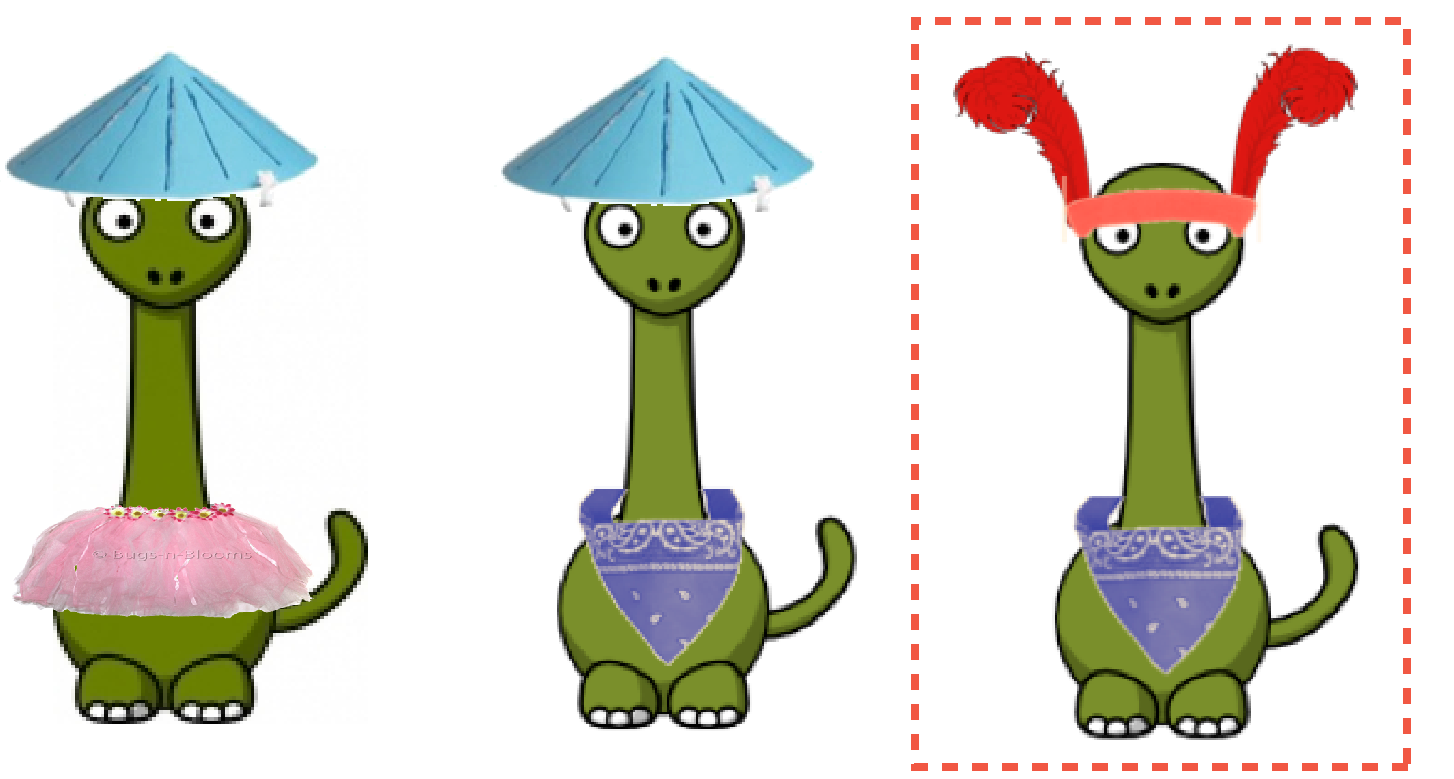
\includegraphics[width=2.5in]{figures/stims_complex.pdf}}}$
\hspace{6ex}
$\vcenter{\hbox{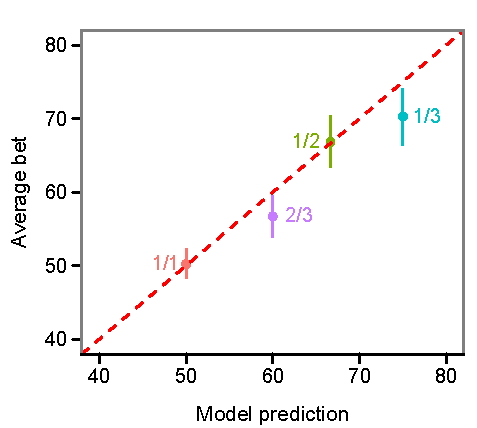
\includegraphics[width=3in]{figures/info_adults.pdf}}}$
\caption{\label{fig:adults} Left: Stimuli for Experiment 1 in a 1/2 trial (see text for description of condition labels). Right: Data from Experiment 1. Points show participants' mean bet with 95\% confidence intervals (computed via non-parametric bootstrap), plotted by the predictions of the informative communication model. The dashed line shows the diagonal (perfect correspondence between predictions and bets).}
\end{center}
\end{figure}


In our analysis, we excluded trials on which participants' bets did not sum to 100 (2.5\% of trials) and on which they failed to answer the check questions correctly (2.9\%). These exclusions did not change the qualitative or quantitative pattern of results. We also verified that there were no effects of object type or target position in a simple linear regression predicting participants' bets (no random effect structure was warranted because each participant contributed only a handful of trials). Thus, we averaged across these aspects of the data and analyzed bets on the target feature by condition. The target feature was designated as the feature that constituted the numerator in the condition name, e.g. the unique feature in 1/2 trials ({\sc headband} in our running example).

\begin{table}
  \begin{center}
    \begin{tabular}{lcccccc}
      \hline
       Trial & Model prediction & $M$ & $SD$ & $t$ & {\it df} & $p$ \\
      \hline
      1/1 & 50.0 & 50.2 & 14.1 & 0.21 & 193 & .83 \\
      1/2 & 66.7 & 66.8 & 23.1 & 10.01 & 189 & $< .0001$ \\
      1/3 & 75.0 & 70.3 & 27.7 & 10.19 & 193 & $< .0001$ \\
      2/3 & 60.0 & 56.7 & 19.8 & 4.65 & 188 & $< .0001$ \\
      \hline
    \end{tabular}
    \caption{\label{tab:adults} Summary statistics and two-tailed one-sample $t$-tests against chance performance (\$50) for each condition in Experiment 1. $M$, and $SD$ denote the mean and standard deviation of bets on the target feature. Degrees of freedom vary from condition to condition due to exclusions (see text for more details).}
  \end{center}
\end{table}



Participants' mean bets on the target feature are plotted by model predictions in Figure \ref{fig:adults}, right, and all data are reported in Table \ref{tab:adults}. The primary prediction in our experiment was that participants' bets would favor the features that were more informative (had smaller extensions). We found that this prediction was satisfied: In the 1/2, 1/3, and 2/3 conditions (all the conditions where there was a difference in extension between features), participants picked the feature with the smaller extension significantly more than chance ($t$-tests are reported in Table \ref{tab:adults}). In addition, all three of these conditions differed significantly from the 1/1 baseline condition (all $p$s $< .001$). Thus, participants in our experiment reliably assigned the meaning of the novel word to the more informative feature of the target object in the context. 

In addition, participants' bets scaled with the relative informativeness of the two features. We found a tight quantitative correspondence between (parameter-free) model predictions and human behavior. When there were equal numbers of objects with each feature, mean bets were very close to \$50, reflecting equal probability. In contrast, in the 1/2 case shown in Figure \ref{fig:adults}, our informativeness model predicted a bet of \$67 in this condition, nearly identical to the participants' average bet of \$67. Although there were only four conditions with distinct model predictions, the correlation between mean bets and model predictions was quite high ($r = .98$, $p = .02$).\footnote{This finding additionally replicates results of an adult experiment reported in \citeA{frank2009b} with a distinct population and stimulus set. In that experiment, which used arrays of six geometric shapes, there were a total of 21 conditions ranging from 1/6 to 5/6, and the overall correlation between model predictions and participants' mean bet was $r=.93$. We conducted this simplified version of the experiment in order to use stimuli more comparable to those used with children in Experiments 2 and 3.} 

Thus, our data suggest that adults' judgments show a quantitative correspondence between the relative informativeness of a property in context and inferences about word meaning. Our next experiments test whether preschool children also show evidence of such sensitivity to informativeness.

%%%%%%%%% EXPERIMENT 2: KIDS %%%%%%%%% 

\section{Experiment 2}

We next asked whether preschool children would also be able to make use of the informativeness of features to learn the meanings of novel adjectives. For this paradigm, we used a simplified version of the 1/2 condition of Experiment 1 that used only two objects and two features, as in our original example in Figure \ref{fig:stims}. 
% Although testing children's quantitative sensitivity to informativeness is an important goal, this first experiment examined only whether children could use a substantial contrast in informativeness to make inferences about word meanings.

\subsection{Methods}

\subsubsection{Participants}

Participants were 24 children from an on-campus preschool, recruited from their classrooms by an experimenter who had previously spent time in their classroom to establish rapport. Children were recruited to fulfill a planned sample of 3 -- 4 year-olds (N=12, mean age = 3;7) and 4 -- 5 year-olds (N=12, mean age = 4;6). 

\subsubsection{Materials and Methods}

Children completed eight total trials, distributed into two conditions: \emph{filler} and \emph{inference}. Inference trials contained two objects: the target object (indicated by a point) had two features, while the distractor object had only one of these (as in the running example shown in Figure \ref{fig:stims}). Filler trials were identical but the target had only one feature, which was not shared with the distractor. For example, a filler version of Figure \ref{fig:stims} would be identical but the target dinosaur would appear without a bandanna, so that the label would unambiguously refer to the headband (because this was the only salient accessory the dinosaur had). Trials were interleaved by condition, with a filler trial always appearing first. 

At the beginning of the paradigm, children were introduced to a stuffed animal named Felix who they were told was visiting a toy store and who they were to help in identifying some new toys. Experimental materials were presented via printed pictures shown in a binder, with training and testing phases shown on subsequent pages. In the training portion of each trial, the experimenter pointed to the target object and said e.g. ``This is a dinosaur with a dax! How neat! A dinosaur with a dax.'' This frame ensured that the target word (``dax'') was spoken twice. The first part of the naming phrase was always ``this is a,'' while the exclamation varied from item to item to provide variety. In the test portion of the trial, children saw two additional images in which one object had each each feature (e.g. a dinosaur with a bandanna only and a dinosaur with a headband only; identical to the filler trials). They were asked ``Here are some more dinosaurs. Which of these dinosaurs has a dax?'' and responded by pointing. 

Materials for the inference trials were identical to those used in Experiment 1; filler trials used monkeys, dogs, cell phones, and cats as the objects. Novel words were ``tupe,'' ``sep,'' ``zef,'' ``gabo,'' ``dax,'' ``fid,'' ``keet,'' and ``toma.'' We counterbalanced trial order, target position in both training and test trials (crossed), and which feature was the target. Features were chosen to be equally salient based on pilot studies using the same paradigm.


\subsection{Results and Discussion}

\begin{figure}[tr]
\begin{center}
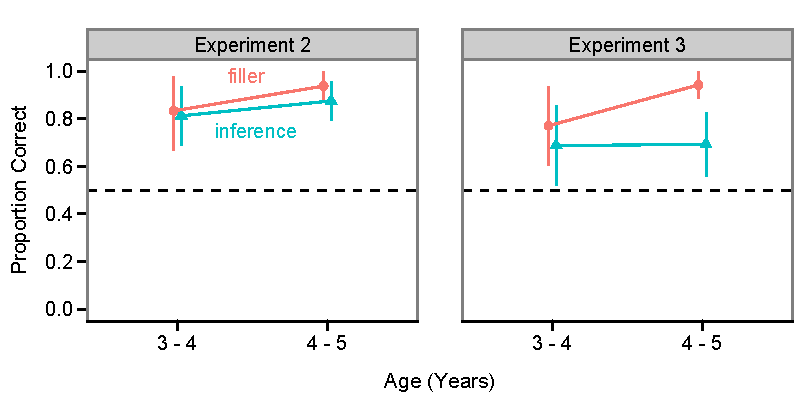
\includegraphics[width=5in]{figures/info_kids.pdf}
\caption{\label{fig:kids} Data from Experiments 2 and 3. Mean proportion correct is plotted by age group for both filler and inference trials. The dashed line shows chance performance. Error bars show 95\% confidence intervals, computed via a non-parametric bootstrap over participant means. }
\end{center}
\end{figure}

If children were able to make use of the relative informativeness of the two possible word meanings, they should choose the more informative word meaning significantly more often than chance. Congruent with this hypothesis, we found that in inference trials, children chose the unique feature (the one that would have been more informative to name in this context) the majority of time (3--4 year olds: M=81\%, SD=39\% and 4--5 year olds: M=88\%, SD=33\%) and nearly as often as they chose the correct feature in filler trials (3--4 year olds: M=83\%, SD=38\% and 4--5 year olds: M=94\%, SD=24\%). Results are shown in Figure \ref{fig:kids}, left. These data suggest that children in our task were sensitive to the contextual distribution of features, even though the literal meaning of the utterance did not strictly rule out the non-unique feature.

To quantify the reliability of this pattern, we fit a logistic mixed effects model to children's responses, with age group and condition as fixed effects, and with random effects of condition fit for each participant and each target item \cite{barr2013}. A model with an interaction term did not provide better fit ($\chi^2(1) = .16$, $p = .69$). The resulting coefficient estimates suggested that three-year-olds (the reference level) were above chance in their responding on inference trials ($\beta = 1.74$, $z = 3.70$, $p = .0002$). There was also a significant coefficient indicating higher performance on filler trials ($\beta = 4.66$, $z=1.92$, $p = .02$). In this study there was no significant effect of age group ($\beta = .47$, $z = .67$, $p = .51$). 

Evidence from this study suggests that children successfully mapped words to features that would have been more likely to be named by an informative speaker. The mean proportion of informativeness-congruent judgements by children in both groups was actually higher than the strict probability assigned by our model (67\%) and higher than that assigned by adults in the betting task in Experiment 1. There are several reasons to be cautious about this kind of quantitative interpretation, however. The context of Experiment 2 was far less stripped down than that of Experiment 1, and the linguistic frame for the novel label encouraged a contrastive reading (something we investigate in Experiment 3). In addition, the two-alternative forced choice measure might have led children to \emph{maximize}, more consistently choosing the highest-probability of the two alternatives  \cite{hudsonkam2005}. Thus, although the evidence strongly points in favor of informativeness, we do not believe a quantitative interpretation is warranted.


%             Estimate Std. Error z value Pr(>|z|)    
% (Intercept)   1.7373     0.4700   3.697 0.000219 ***
% age.group4    0.4703     0.7070   0.665 0.505928    
% typefiller    4.6561     1.9157   2.430 0.015082 *  


\section{Experiment 3}

As mentioned above, one question about the findings of Experiment 2 comes from the use of the contrastive sentence frame ``This is a dinosaur with a dax.'' The deictic ``this'' is, in the terminology of \citeA{clark2002}, a ``direct offer''---the use of a deictic term for the exclusive purpose of providing a label. This exclusive purpose may have given participants a greater sense that the utterance should be chosen with maximal informativeness. In addition, the deictic ``this'' is easy to stress contrastively, implying to listeners that ``this [and not that other one] is a dinosaur with a dax.'' 

In Experiment 3, we replicated the methods of Experiment 2 exactly but used the frame ``here is a'' instead. By virtue of its focus on location, rather than identity, ``here is a'' provides an alternative goal for the utterance: establishing in the common ground the location of a particular dinosaur \cite{clark1996}.  In addition, in Experiment 3, we avoided the strong prosodic phrase boundary between ``here'' and ``is'' that would be necessary to imply contrastive stress in this condition (e.g. ``here... is a dinosaur with a dax''). A mapping of ``dax'' to the unique feature in this study would imply that the results of Experiment 2 are not specific to a single construction type. 

\subsection{Methods}

\subsubsection{Participants}

Participants were 25 children from the same on-campus preschool as Experiment 2. Children were recruited to fulfill a planned sample of 3 -- 4 year-olds (N=12, mean age = 3;8) and 4 -- 5 year-olds (N=13, mean age = 4;3).

\subsection{Materials and Methods}

Materials and methods for Experiment 3 were identical to those in Experiment 2 except that we replaced the naming phrase ``This is a'' with the phrase ``Here is a.'' 

\subsection{Results and Discussion}

Results are shown in Figure \ref{fig:kids}, right. Overall, performance in the inference trials was lower than in Experiment 2, but was still above chance (3--4 year olds: M=69\%, SD=47\% and 4--5 year olds: M=69\%, SD=47\%). Filler trial performance remained quite high (3--4 year olds: M=77\%, SD=42\% and 4--5 year olds: M=94\%, SD=24\%). 

We again applied logistic mixed effects regression, though in this case we retained the interaction between condition and age because it increased model fit. We found that three-year-olds in the inference condition were significantly above chance ($\beta = .93$, $z = 2.17$, $p = .03$), and there was no main effect of age group ($\beta = .04$, $z = .06$, $p = .95$). Performance on filler trials was higher than on inference trials, though not significantly so ($\beta = 1.04$, $z = 1.42$, $p = .15$), but there was a marginally significant interaction of trial type and age group ($\beta = 2.02$, $z = 1.64$, $p = .10$). This interaction suggests that the age-related increase in filler trial performance was not seen reliably in the inference trials---both 3--4 and 4--5 year olds were above chance, but they were not even numerically different from one another. 

Although children's performance was numerically lower in the inference trials in Experiment 3 than it was in Experiment 2, we nevertheless replicated the use of informativeness to make inferences about word meaning. Either the ``this is a'' construction or the stress with which it was marked likely contributed to the somewhat higher level of inferences in Experiment 2, and in naturalistic situations, these information sources both likely scaffold children's performance in making similar inferences. But even in their absence, children still appeared to notice the differential informativeness of the unique feature and treat that property as the extension of the novel word. 

%   age.group      type   correct
% 1         3    filler 0.7708333
% 2         4    filler 0.9423077
% 4         3 inference 0.6875000
% 5         4 inference 0.6923077

% > aggregate(correct ~ age.group + type,d2,sd)
%   age.group      type   correct
% 1         3    filler 0.4247444
% 2         4    filler 0.2354355
% 4         3 inference 0.4684174
% 5         4 inference 0.4660414



%%%%%%%%% CONCLUSIONS %%%%%%%%% 
\section{General Discussion}

We began by revisiting a fundamental question in language acquisition: How do children infer the meanings of words in ambiguous situations? Although a variety of partial answers to this problem have been identified by prior research, a large class of situations (including some construals of Quine's famous problem) are not addressed by these. We have argued here that in some of these cases, word meaning can be disambiguated by the combination of knowledge of speakers' communicative goals and the assumption that they are using language informatively to achieve those goals \cite{grice1975}. Our contributions here are then to formalize this inference using a model of pragmatic reasoning and to show that adults and children are able to use contextual informativeness in simple situations to infer word meanings.

In our prior work, we described a framework for pragmatic inference that can be used to make predictions about the behavior of speakers and listeners in simple reference games \cite{frank2012}. As we showed here, this framework can also be extended straightforwardly to make predictions about what novel words should mean, given that they are uttered by an informative speaker.  We then tested predictions from this framework. In Experiment 1, we showed that the aggregate judgments of adult learners conformed quantitatively to the predictions of the pragmatic computation we described. In Experiments 2 and 3, we provided evidence that preschoolers' also made use of contextual informativeness in word learning inferences. Together these data suggest that adults and children can use Gricean considerations to infer word meaning in otherwise ambiguous situations. 
% In fact, perhaps the strongest evidence of this result is that situations like Figure \ref{fig:stims} do not \emph{seem} ambiguous at all. 

Our work builds on a long tradition of considering pragmatic reasoning in early language learning \cite{clark2003,bloom2002,tomasello2003}. Some of its closest antecedents come from early work on the role of pragmatics in young children's language, where Greenfield, Bates, and their colleagues developed the notion of informative use in context \cite{bates1976,greenfield1976,greenfield1978}. These authors were interested in how children chose which aspects of the world to label using their early language. They posited that children chose the most informative element of a situation and encoded it in speech. 

Yet many of the ideas in this work did not see extensive further development. In a critique of this work, \citeA{pea1979} noted that

\begin{quote}
the term 'informativeness' is defined in loose \emph{pragmatic} terms... yet no pragmatic theory of information, with the intricacies which would be required in incorporating the belief-states of [speakers] A and B and their changes over time, has ever been developed. ... So the allusion to a formal pragmatic information theory is based on an illusion. (p. 406--407)
\end{quote}

\noindent Pea's comment highlights a key weakness of these early approaches: they had no formal framework in which to ground observations about pragmatics. Our work here revisits the same set of questions posed in this earlier work (although from the perspective here of language learning as well as language use): how can we formalize powerful Gricean notions of informativeness in context such that it can be applied to make quantitative predictions? We believe that the use of formal models points the way forward for further investigations of children's pragmatic abilities in early learning.


Our data leave open the question of the psychological mechanisms by which adults and children compute the informativeness of a word in context. We note two particular issues here. First, we cannot differentiate between the case in which each participants' judgments are slightly affected by aspects of the contexts and the case in which some participants notice the informativeness of a feature and others do not. This is a general issue in translating computational-level models of human cognition to the psychological process level \cite{frankinpressb}. 

Second, and more specific to the particular domain at hand, it may be that the relative infrequency (uniqueness) of the most informative feature draws attention to it. We have not attempted to differentiate this psychological explanation experimentally because, to a first approximation, unique features, objects, and events are in fact more likely to be referred to. Thus, the same mechanisms that draw our attention to the unexpected, surprising, and rare may be those that help us decide what is informative to talk about. The degree to which children (or adults) take others' perspective in judging the novelty of a stimulus is an open question. Experiments on discourse novelty suggest some degree of perspective-taking \cite{akhtar1996}, but it is controversial even for adults the degree to which others' perspectives are considered in language comprehension \cite{keysar2003,nadig2002,brown-schmidt2008}. Thus, this topic will be a fruitful direction for future work.

Children can make many partial solutions to the Quinian \citeyear{quine1960} puzzle of ambiguity, employing strategies from cross-situational observation to disambiguation with prior linguistic knowledge, and such strategies can be very helpful. Yet there are still many examples where they fail, including the cases studied here. We have argued that cases where other strategies fail may still be disambiguated by considering the speaker's pragmatic goals. In fact, as we have argued elsewhere \cite{frank2009}, this consideration of the speaker's communicative goals may form a broader strategy for language acquisition, accounting for other phenomena as a byproduct of statistical inference over social representations. 

\newpage

\bibliographystyle{apacite}
\bibliography{icom}

\end{document}

